\subsection {Sprint 2}

A \textit{sprint} 2 foi caracterizada pela realização de ajustes e correção de comportamentos inesperados que surgiram durante os testes de aceitação das funcionalidades entregues na \textit{sprint} 1, conduzidos pelo time de produto. Os trabalhos começaram assim que a lista de ajustes necessários foi levantada, e pode ser sumarizada nos seguintes requisitos:

\begin{itemize}
	\item \textbf{Requisito 1 da Sprint 2}: Corrigir problema onde um parágrafo que possua trechos em itálico e negrito são erroneamente divididos em mais de um parágrafo;
	\item \textbf{Requisito 2 da Sprint 2}: Corrigir problema de imagens quebradas quando copiadas do Google Docs ou Microsft Word;
\end{itemize}

\subsubsection {Requisito 1 da Sprint 2}

Alguns parágrafos que possuiam itálico e negrito em seu conteúdo, eram erroneamente divididos em multiplos parágrafos. Por exemplo o \textit{input} HTML:

\begin{table}[h]
	\begin{tabular}{c}
		\texttt{<h1>Título do Texto</h1>}\\
		\texttt{<div>}\\
			\texttt{Parágrafo! <strong>Aqui vem o conteúdo</strong>}\\
			\texttt{do parágrafo do usuário.<br>}\\
			\texttt{Aqui é outro parágrafo.<br>}\\
		\texttt{</div>}\\
	\end{tabular}
\end{table}

seria dividido em cinco parágrafos:

\begin{itemize}
	\item \texttt{<h1>Título do Texto</h1>};
	\item \texttt{Parágrafo!};
	\item \texttt{<strong>Aqui vem o conteúdo</strong>};
	\item \texttt{do parágrafo do usuário.};
	\item \texttt{Aqui é outro parágrafo.}.
\end{itemize}

Isso acontece devido ao fato de que no Nokogiri, texto puro também é tratado como um nó na árvore do documento XML/HTML. Ao fazer a tratativa de separar as \texttt{<div>} exibida na Figura \ref{fig:trix-paragraph-split}, o método \texttt{\#children} separará o primeiro parágrafo em três, pois entende-se que a \textit{tag} \texttt{strong} é um elemento independente na árvore. A Figura \ref{fig:arvore-nokogiri-problema-italico-negrito} ilustra o comportamento.

\begin{figure}[htbp]
  \centering
  \caption{Diagrama representando a árvore do HTML após o \textit{parsing} do Nokogiri}
  \label{fig:arvore-nokogiri-problema-italico-negrito}
  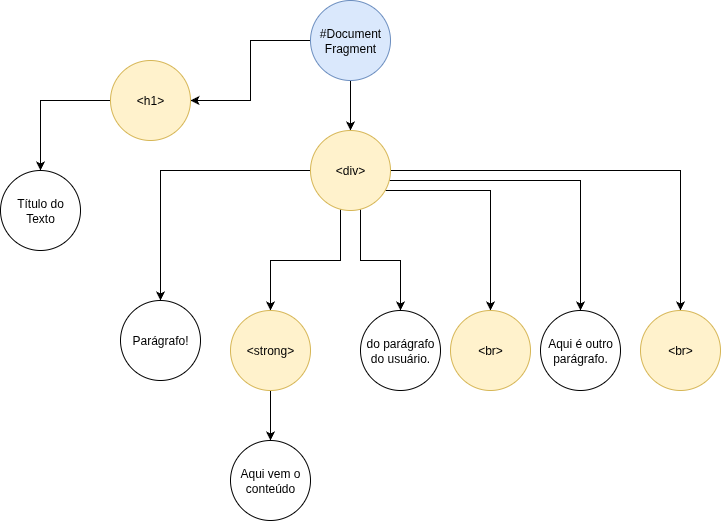
\includegraphics[width=\textwidth]{figuras/arvore-nokogiri-problema-italico-negrito.png}
  \fonte{Próprio autor}
\end{figure}

Para resolver esse problema, foi criado um método para fazer a extração dos parágrafos com base nos filhos diretos de uma \texttt{<div>}, onde dois ou mais filhos podem ser considerados pertencentes ao mesmo parágrafo. O critério para dividir os nós filhos entre mais de um parágrafo é o aparecimento de um elemento \texttt{<br>} entre eles. A Figura \ref{fig:diagrama-metodo-split-nokogiri} mostra como a divisão ocorre na visualização de árvore. Caso seja encontrado um elemento \texttt{<div>}, seus filhos serão agrupados até que se encontre o elemento divisor (\texttt{<br>}). Os elementos são analisados da esquerda para direita. Esse método foi inserido diretamente na classe \texttt{Nokogiri::XML::Nodeset} na inicialização da aplicação. A Figura \ref{fig:metodo-split-nokogiri} mostra a implementação e o uso.

\begin{figure}[htbp]
  \centering
  \caption{Diagrama representando o agrupamento de elementos filhos separados por \texttt{<br>}}
  \label{fig:diagrama-metodo-split-nokogiri}
  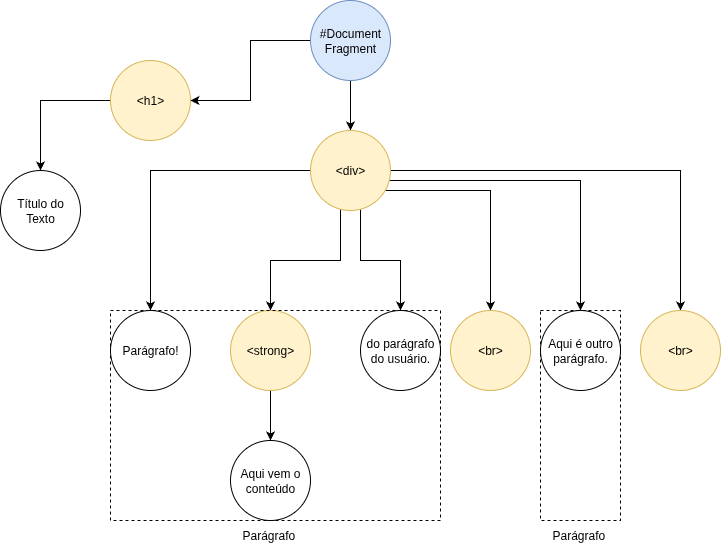
\includegraphics[width=\textwidth]{figuras/diagrama-metodo-split-nokogiri.png}
  \fonte{Próprio autor}
\end{figure}

\begin{figure}[htbp]
  \centering
  \caption{Definição e uso do método \texttt{split}}
  \label{fig:metodo-split-nokogiri}
  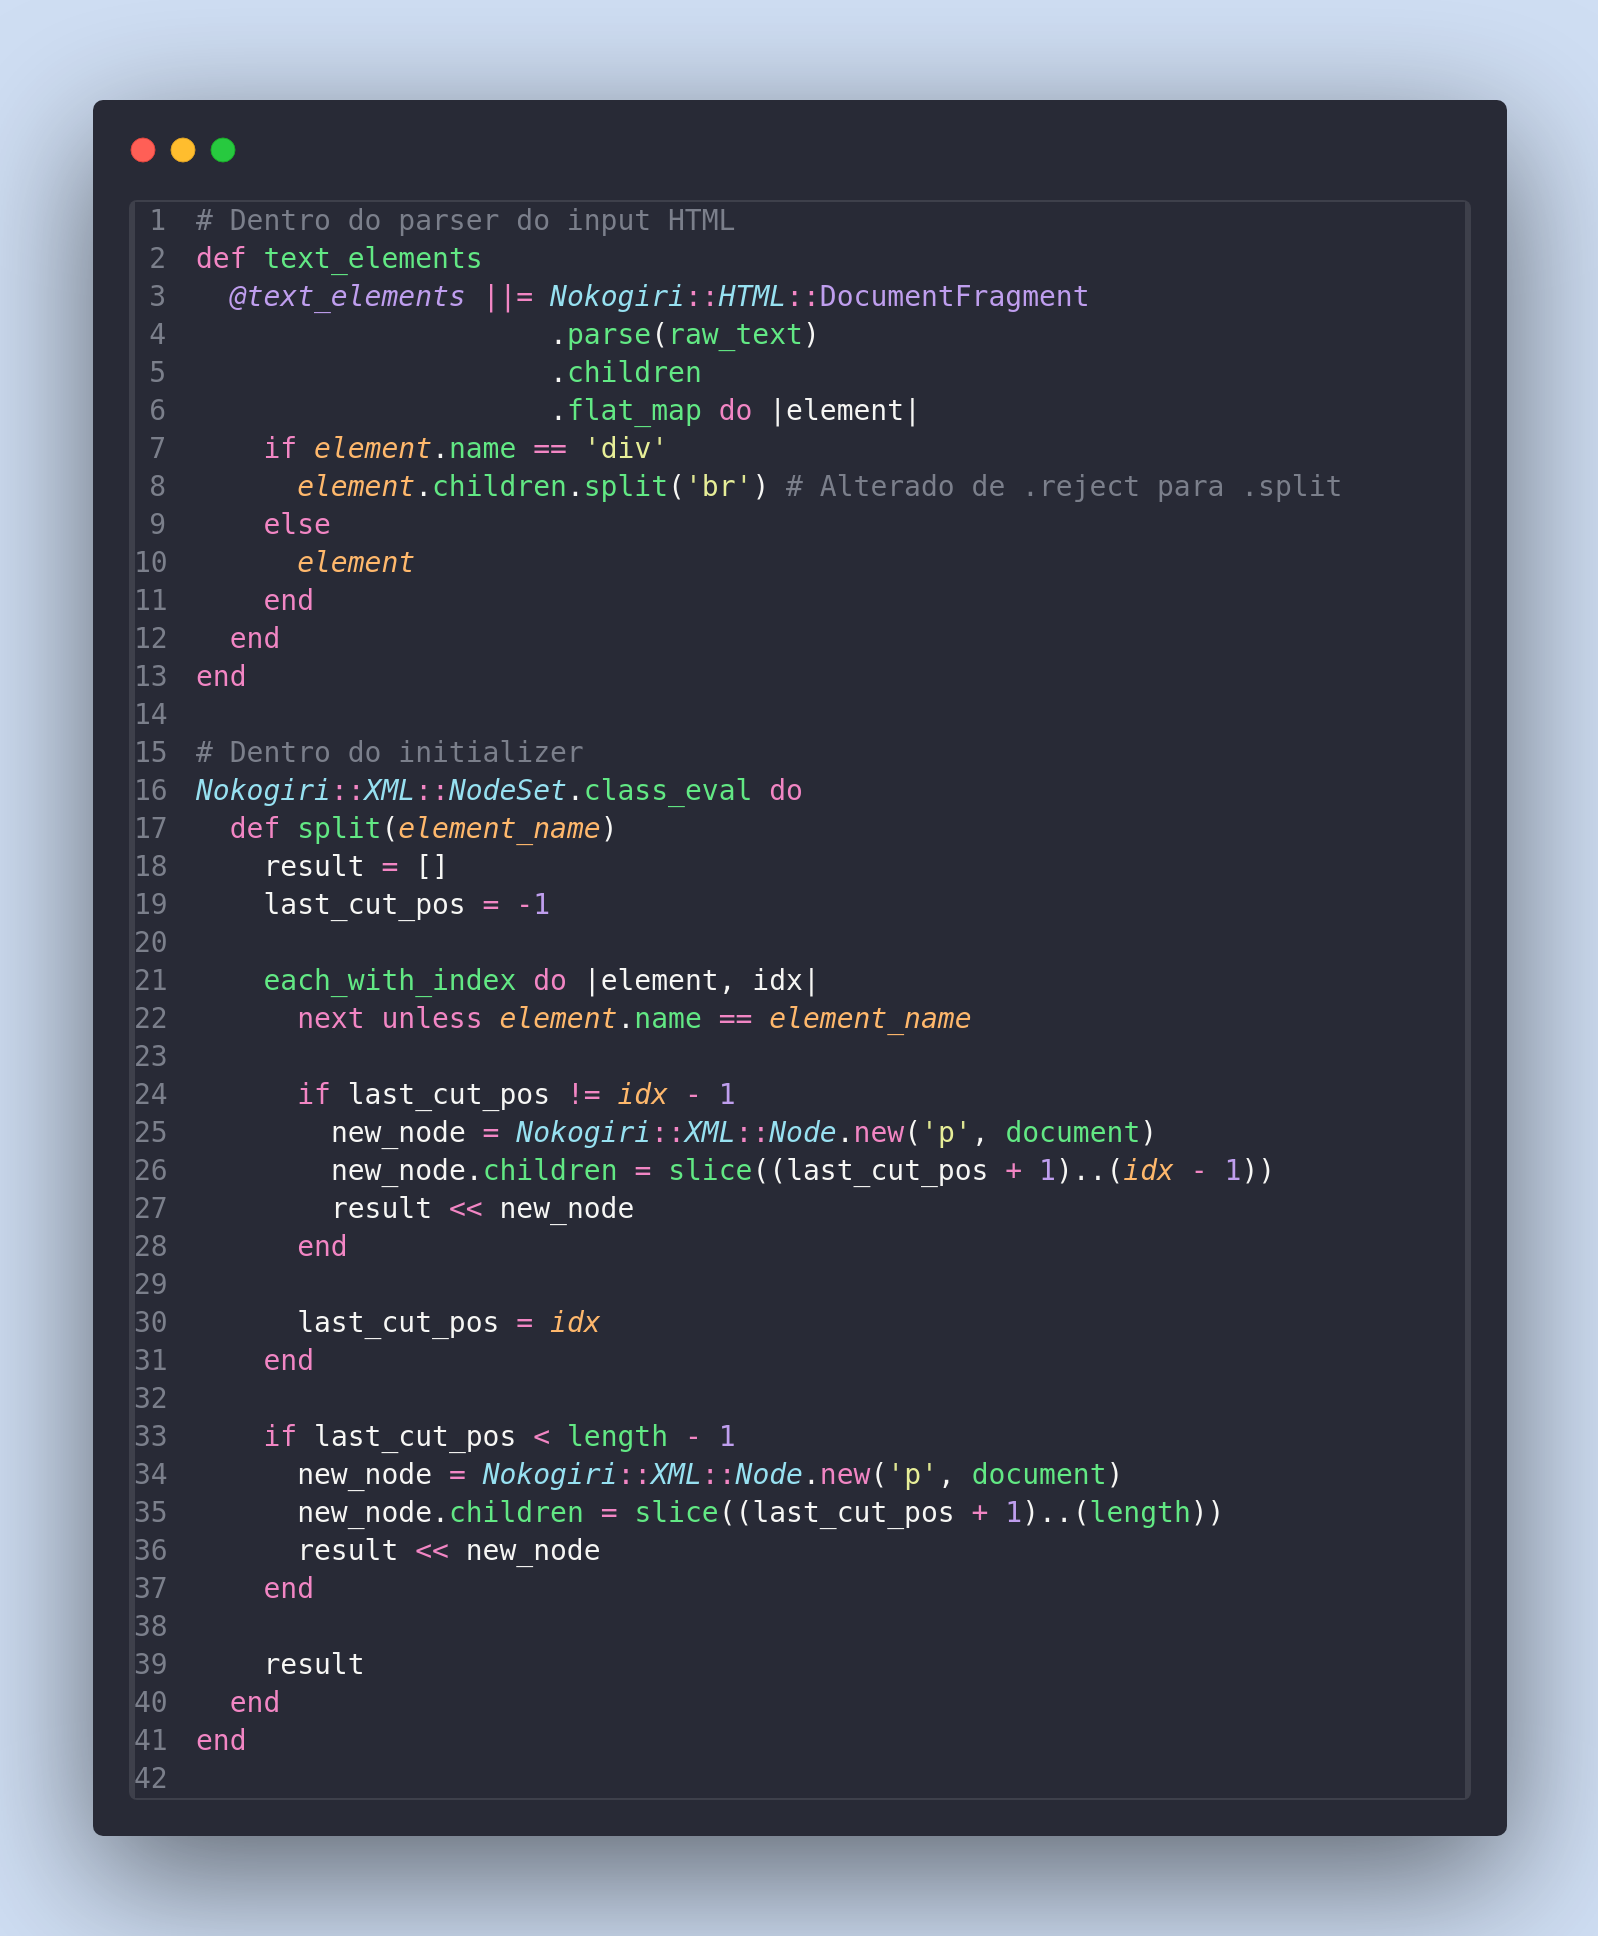
\includegraphics[width=\textwidth]{figuras/metodo-split-nokogiri.png}
  \fonte{Próprio autor}
\end{figure}

\subsubsection {Requisito 2 da Sprint 2}

Ao utilizar o comando copiar em editores de texto como o Google Docs, na maioria das vezes o conteúdo da imagem em si não era copiado, mas sim um \textit{link} para onde ela está guardada. Para esses casos, a imagem (\texttt{<img>}) já era inserida no texto com o seu atributo \texttt{src} preenchido, e não era automaticamente enviada para o \texttt{storage} do \textit{Rails}, pois o seu conteúdo (\texttt{blob}) sequer estava lá.

Para resolver esse problema, uma das possibilidades seria fazer uma requisição para a fonte da imagem, para em seguida enviá-la para o \texttt{storage} usando a \textit{controller} \texttt{Attachments}. Mas, essa alternativa tinha dois problemas: barreiras com o \textit{Cross-Origin Resource Sharing} (CORS), e disponibilidade limitada do recurso.

CORS é um mecanismo para controle de requisições entre domínios distintos quando a requisição é feita pelo \textit{browser}, fazendo com que nem sempre o Brasil Participativo tenha permissão para baixar imagens de outras fontes automaticamente \cite{cors-explanation}.

Outra possibilidade seria deixar o elemento HTML que representa a imagem intocado e referenciando o \textit{link} externo mesmo depois de salvar o parágrafo no banco de dados. Porém, algumas fontes possuem mecanimos de \textit{throttle} para impedir que uma determinada origem faça requisições demais, além de que não há garantias de que o recurso estará disponível a qualquer instante que se queira buscá-lo.

Portanto, para garantir a consistência na inserção de imagens no texto, o usuário não conseguirá mais inserir imagens através do comando copiar e colar. Será necessário manualmente baixar a imagem no computador e inserí-la no corpo do texto, seja arrastando, seja utilizando a funcionalidade de upload de arquivos do Trix.

Para realizar esse comportamento, foi escrito uma nova customização no Trix para observar o evento \texttt{trix-before-paste}, que é disparado antes do conteúdo ser inserido no \textit{input}. Caso seja detectado algum elemento de imagem no conteúdo colado, este será substituído por uma mensagem de aviso, além de alertar o usuário com uma mensagem do próprio navegador de que ele deve seguir outro procedimento para realizar a inserção daquela imagem. Na Figura \ref{fig:trix-removendo-imagens} é exibido o código JavaScript que realiza essa verificação.

\begin{figure}[htbp]
  \centering
  \caption{Código JavaScript para remover imagens inseridas através do copiar e colar}
  \label{fig:trix-removendo-imagens}
  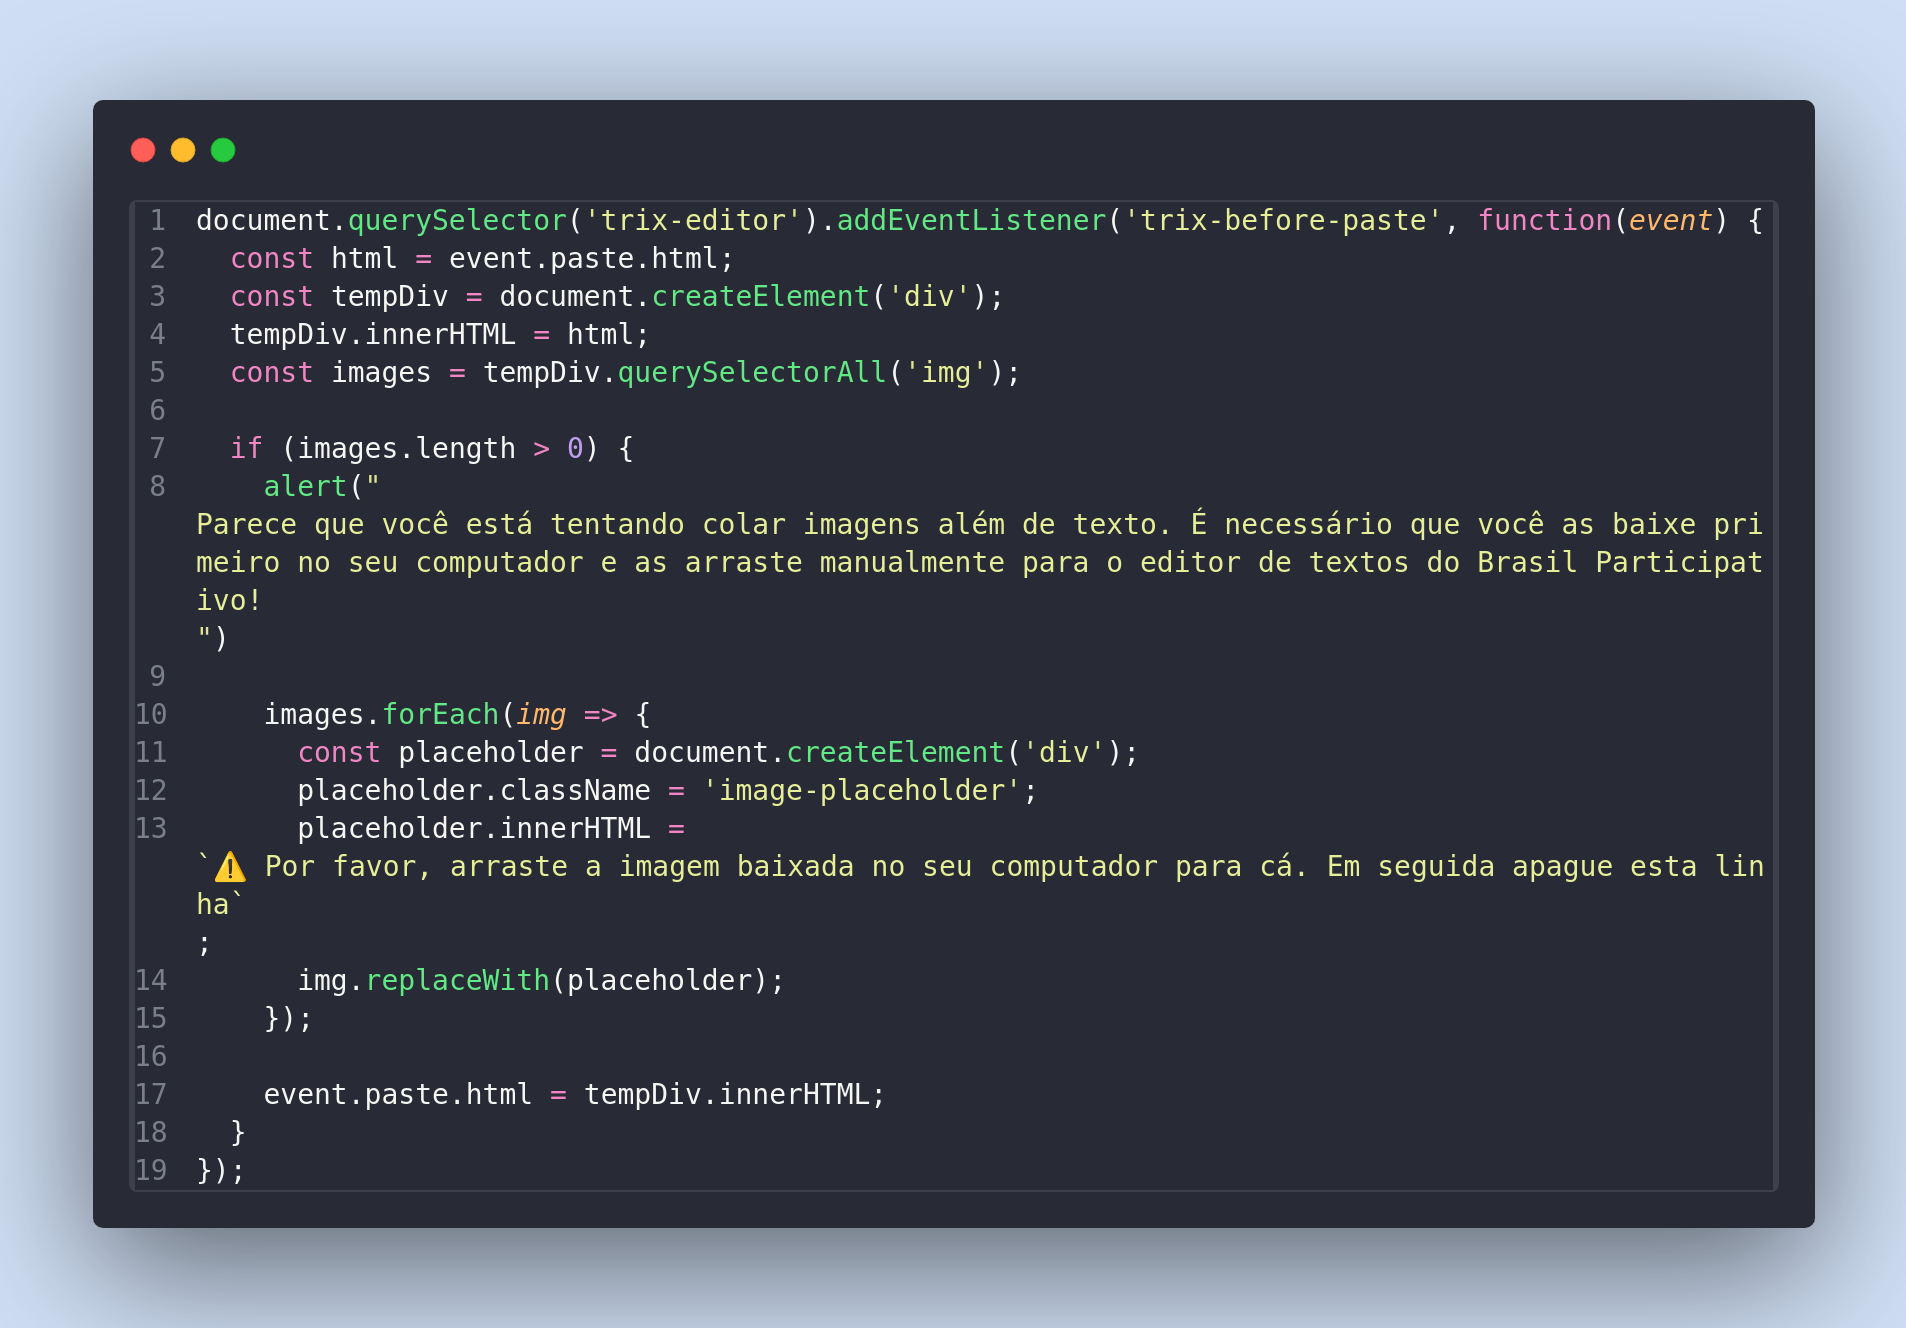
\includegraphics[width=\textwidth]{figuras/trix-removendo-imagens.png}
  \fonte{Próprio autor}
\end{figure}